%!TEX root = ../thesis.tex
%*******************************************************************************
%****************************** Second Chapter *********************************
%*******************************************************************************
\ifpdf
    \graphicspath{{Chapter2/Figs/Raster/}{Chapter2/Figs/PDF/}{Chapter2/Figs/}}
\else
    \graphicspath{{Chapter2/Figs/Vector/}{Chapter2/Figs/}}
\fi
\chapter{Measuring fluctuating asymmetry from long term field sites: A case study on \textit{Pongo} spp.}

Fluctuating asymmetry is a random non-directional deviation in symmetry on bilateral features caused by developmental instability. Previous studies have indicated that elevated levels of fluctuating asymmetry are correlated with negative health outcomes and reduced perceived attractiveness. It has been suggested that secondary sexual traits may be more sensitive to fluctuating asymmetry due to their high metabolic cost and subsequent use as an unbiased indicator of fitness. In this study, I use historic long term photographic data sets from two field sites to examine the variance in facial fluctuating asymmetry in flanged males across two sub-populations, and examine whether fluctuating asymmetry in flanges can be observed. Composite relative fluctuating asymmetry scores were higher in the Bornean field site compared to the Sumatran field site, which I suggest may be due to the lower overall fruit availability and comparatively poor ecological health of the Bornean field site. Flange measurements showed poor repeatability between photos taken on different days, which I suggest may be in part due to significant flange plasticity over time after their development. This study indicates the usefulness of historic photographic data sets for examining changing ecological conditions and their implications on wild animal health.
 \pagebreak

\section{Introduction}
Biologists differentiate between 3 types of asymmetry: Directional asymmetry, antisymmetry, and fluctuating asymmetry (FA) (Fig. \ref{fig:examplefaplots}). Directional asymmetry (DA) is where a trait value is larger on one side of the body compared to the other across a population, for example, in humans the right gonad tends to be larger than the left \citep{MITTWOCH.1975}. In contrast, antisymmetry (AS) is where the trait value is asymmetric, but there is no preference of which side is larger across a population \textit{i.e.} it can be larger on either side of the body \citep{Zakharov.20223bp}. For example, largemouth bass show AS in their limb usage and turning direction which is maintained through negative frequency-dependent natural selection as their prey (freshwater gobies) are also antisymmetric \citep{Yasugi.2012}. While both DS and AS can have fitness benefits in specific organisms and result from normal development, fluctuating asymmetry (FA) is an indicator of developmental instability \citep{Valen.1962}.


\begin{figure}[h]
    \centering
    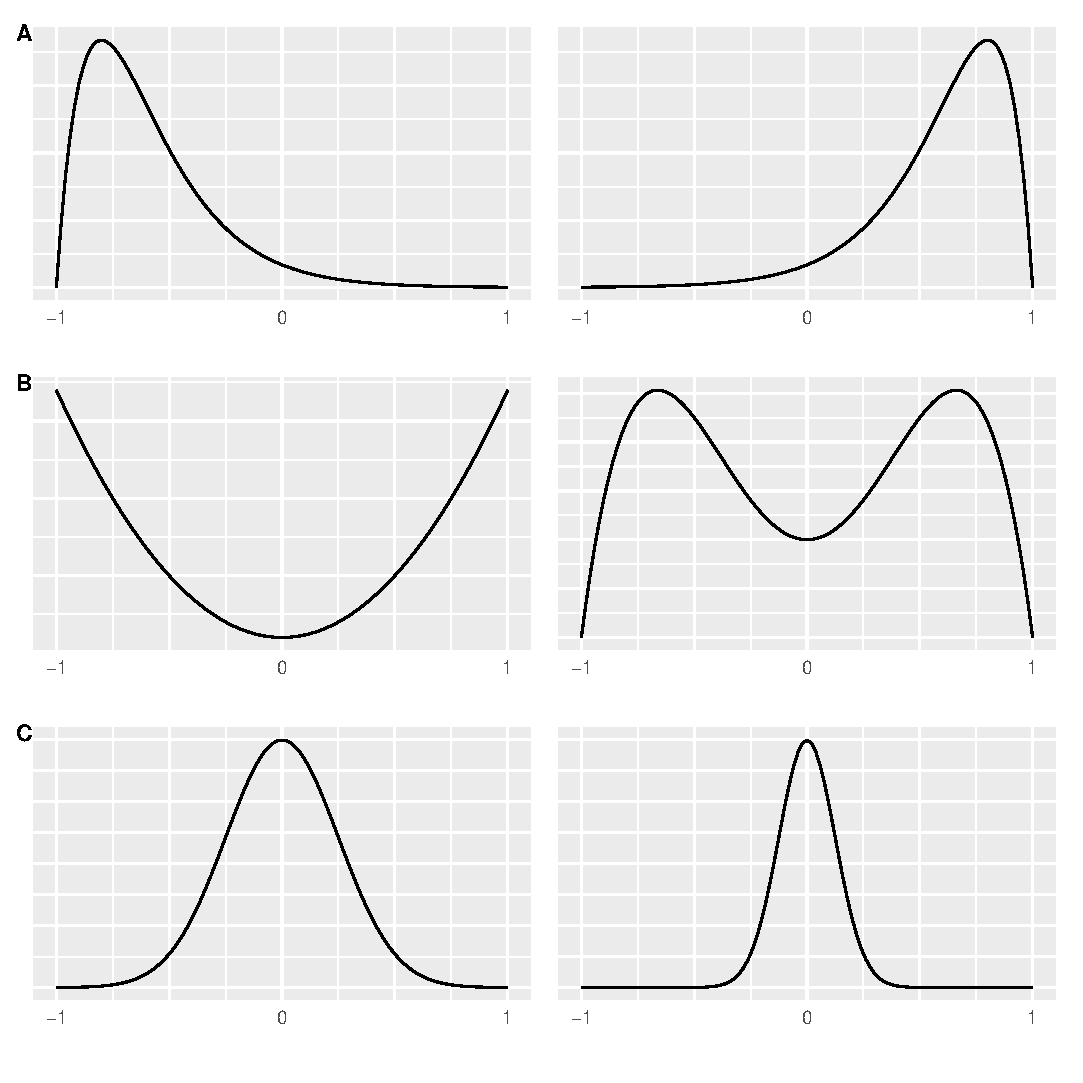
\includegraphics[width=0.75\textwidth]{Chapter2/Figs/Vector/spee.eps}
    \caption{Example population trait values under different types of asymmetry. 
A. Directional asymmetry. 
B. Antisymmetry. 
C. Fluctuating asymmetry. }
    \label{fig:examplefaplots}
\end{figure}

\pagebreak
Fluctuating asymmetry (FA) is minor non-directional deviance in trait values from perfect bilateral symmetry and is caused by environmental or genetic developmental instability (DI) \citep{Palmer.1986}. The presence of FA across organisms has been shown in laboratory conditions and in the wild across organisms and stressors. These stressors can be environmental (e.g., low food availability, pollution, social stress) or genetic (e.g., hybridisation, genetic disorders, inbreeding) \citep{Beasley.2013, Leung.1996, VØLLESTAD.1999}. In insects, meta-analyses have shown that FA is a sensitive biomarker to environmental stress across a variety of different traits, and is caused by a variety of stressors. However, the sensitivity of a particular trait to a specific stessor varied between different traits \citep{Beasley.2013}. Given the cost of maintaining homeostatic development, buffering against FA is likely to be prioritised in traits vital for survival \textit{e.g.} symmetry in leg length is important for efficient locomotion. Therefore, traits of relatively low functional importance are likely to experience more FA compared to vital ones, even under low external stress \citep{Leung.1997}. Together, these meta-analyses highlight the importance of trait selection when measuring FA, with attention paid to the particular ecology and functional role of each trait \citep{Landi.2021}.

At the population level, higher FA scores are more common in populations undergoing stress, meaning that FA could be used as a tool to monitor anthropogenic impacts on animals. Several studies have supported this assertion. In mammals, \citet{Kucheravy.2022} has shown an increase in FA of whisker spots in polar bears since 2003, which correlates with significant habitat degradation due to climate change. In birds, wing and tarsus FA was found to be significantly higher in forest fragments compared to continuous forest in 100 different species in the Brazilian south eastern Atlantic rainforest \citep{Anciães.2000}.  FA could also be used as a method of monitoring threatened populations, previous studies on Cuvier's gazelle have shown that increased levels of FA in horn length are strongly correlated with the coefficient of inbreeding, which in turn is strongly correlated with the proportion of abnormal sperm in the ejaculate \citep{Roldan.1998}. 

In addition to wild animals, FA is an important tool for monitoring captive or managed populations. Zoo animals are often endangered and managed populations generally have significantly lower genetic diversity compared to wild populations. Low genetic diversity has been associated with increased levels of FA in many organisms \citep{Leary.1989}. In healthy populations FA has very low heritability; however, it has been hypothesised that epistasis caused by low population genetic diversity, hybridisation between species, or rapid environmental change can cause additive genetic variation for FA, which in turn reduces the ability of populations to buffer against environmental change \citep{Leamy.2005}. As such, it has been suggested that populations with small effective population sizes are more sensitive to FA caused by environmental stress \citep{Knierim.2007}. This has been observed across gorilla subspecies, where facial asymmetry mirrors known genetic diversity, with significantly inbred mountain gorillas showing significantly higher facial FA compared to western lowland gorillas \citep{McGrath.20220bl}.

\subsection{Fluctuating asymmetry as a measure of health}
Multiple studies have linked increased fluctuating asymmetry in primates with negative health outcomes, however, this issue is controversial (see Section 2.1.2). 

In western lowland gorillas, canine FA correlated strongly with both the year of collection, due to increased human encroachment into their habitat, decreasing the availability of high-quality food resources \citep{Manning.1994}. In captive chimpanzees, facial FA was positively correlated with zookeeper reports of negative physical and mental health symptoms \citep{Sefcek.2007akp}.
Some of these relationships have also been seen in humans, \citet{Thornhill.2006} found that increased levels of body FA were correlated with self-reported health issues. Furthermore, increased levels of fluctuating asymmetry has also been linked to higher BMI in women, and the number of reported health conditions in both sexes \citep{Milne.2003, Al-Eisa.2004}. Notably however, there appears to be no link between FA and a number of common indicators of overall health in recent studies, including cardio-respiratory fitness, blood pressure, or blood cholesterol levels \citep{Milne.2003, Thornhill.2006, Dongen.2011}. This may be in part due to the minimisation of environmental stressors in modern western societies, which makes the underlying FA too small to measure. In contrast, bioarcheological studies on historic human cranial FA have indicated previous links between malnutrition and cranial FA in several different locations around the world \citep{DeLeon.2007,Dongen.2011,Jung.2016}.

\subsection{Issues with fluctuating asymmetry as a measure of health}
Whether FA can be universally used as a useful tool for monitoring population health has been questioned, for two notable reasons. 

Firstly, there is the inconsistency in studies regarding the relationship between FA and sexual selection, health, and individual condition. While meta-analyses have been published showing small but significant relationships between FA and population health and environmental stressors, individual studies are still mixed on the relationships between FA and population/individual outcomes.  This may be in part due to poor trait selection; as it has been hypothesised that sexually selected traits may undergo greater levels of FA compared to nonsexually selected traits, however, previous meta-analyses have not shown such a relationship. However, this inconsistency may also be due to the nature of FA itself, as the variance in trait position/size measured using FA studies is very small (typically <1\% of overall trait size). This increases the impact of measurement error (ME) which both reduces statistical power on analyses and masks effect sizes. Although today the relationships between FA and fitness, stress, and developmental instability are not generally challenged, individual FA studies do not consistently display this relationship, as it is either too weak a relationship, non-existent, or masked by analytic analysis.

Secondly, there is the role of publication bias, the tendency of positive results to be published over negative results. This bias may cause an overestimate of the effect size of any impact between FA and a given outcome, while the true effect size may be much smaller, if present at all. Publication bias is not unique to FA studies, and while in general it is not intended to deceive readers, the tendency of authors to submit positive results and the tendency of journals to publish positive results lead to the publication of effect sizes larger than the true mean effect \citep{Levine.2009}. One of the methods for examining publication bias can be identified by examining a range of papers on the relationship between effect size and sample size. Smaller sample sizes are more likely to contribute to publication bias as the significance threshold is reduced compared to those with larger sample sizes, and studies with small sample sizes with no observed relationship are less likely to be published compared to those that show a significant relationship or negative studies with large sample sizes. A recent meta-analysis of human FA in relation to a variety of health outcomes (disease, psychological maladaptation, reproductive outcomes and attractiveness) indicated that effect sizes co-varied negatively with sample size, which is indicative of publication bias \citep{Dongen.2011}. This relationship has also been observed in other meta-analyses of FA studies with respect to sexual selection \citep{Palmer.1999}.
Furthermore, there can be a relationship between the year of publication and publication bias, as there is an observed tendency for negative results to not be published for a given biological question until positive results have been first published ( \textit{i.e.} there is preferential treatment of initial positive results). Notably, this was not observed in \citet{Dongen.2011}'s meta-analysis of human FA and health outcomes, but has been observed in relation to FA and sexual selection, where the year of publication negatively co-varied with the proportion of positive results published \citep{Tomkins.2003}.

\subsection{Sexual selection, fluctuating asymmetry and the role of faces in primate signalling}
Sexual selection provides an important evolutionary perspective on behaviour and fitness in biology. \textit{Fitness indicator theory }is a subset of sexual selection and suggests that external phenotypic traits can be unbiased indicators of an individual's fitness \citep{Zahavi.1975}. In the traditional 'good genes' model, the male has a secondary sexual ornament which is homeostatically costly to maintain and detrimental to survival. The magnitude, colour, or symmetry of the trait then provides an unbiased indicator of the individual's ability to buffer against environmental instability, such as reduced food availability or pathogen pressure. The trait then spreads through the population as the trait and the preferences are inherited. Over time, this strong directional selection may lead to the trait and preference alleles becoming fixed. This provides fitness benefits to the sender and receiver of the signal, as producing a high-quality trait increases the sexual fitness of the sender, and the receiver benefits from being able to decide the choice of partner from differences in this trait \citep{Zahavi.1977}.

Given the correlation between FA and overall fitness, combined with the pressures of anisogamy, it is likely that there is increased pressure for females to recognise FA in their mating partners even in species without conspicuous signals \citep{Palmer.1986}. Furthermore, given the costly nature of honest fitness signalling, these traits are more likely to be subject to FA compared to purely functional traits \citep{Beasley.2013, Vijendravarma.2022}. This link between sexually selected traits and increased sensitivity to FA has been observed in multiple species across different taxa \citep{Thornhill.2006, Little.2008, Little.2012, Beasley.2013}. 

Among primates, one of the most important mediums for communication and signaling is the face. The face can be used to communicate individual identity, age, gender, emotion, and in some sexually dimorphic species, resource holding potential \citep{Setchell.2001}. Some species of guenons use facial coloration to differentiate between their own species and sympatric heterospecifics \citep{Caro.2005}. Individual facial recognition varies among primates and seems to depend in part on their social structure and in part on their body size \citep{Parr.2011}.  Many primates show facial sexual dimorphism: significant cranial sexual dimorphism is seen in the crania of macaques, mandrills, and white-eyelid mangabeys \citep{O'Higgins.2002}. This dimorphism can include conspicuous facial adornments, notably proboscis monkeys, in which the size of their noses positively correlates with their likelihood of winning antagonistic interactions despite negatively correlated with the size of their canines \citep{Matsuda.2020g6t}. In humans, some studies have indicated that males with more masculine faces may tend to be more dominant in Western cultures \citep{Swaddle.2002}. However, while there is debate as to whether human male masculinity is an honest indicator of fitness outside of mating success, some studies have indicated a correlation \citep{Fink.2007, Dongen.2014}. In particular, facial masculinity has been negatively correlated with the duration of respiratory infection and the number of acquired infections \citep{Dongen.2011}. 

Facial symmetry plays a significant role in mate choice across primates, as there is strong evidence of a conserved preference towards symmetrically faced partners. In rhesus macaques, females show a preference for digitally altered symmetric faces compared to asymmetric ones \citep{Waitt.2006}. This relationship has also been observed in humans, it has been shown that humans rate digitally altered symmetrical faces as more attractive than their real counterparts, and this preference for symmetrical faces is conserved across many cultures \citep{Perrett.1999,Little.2007,Little.2008}. 
This may be because the underlying mechanisms controlling sexual dimorphism and symmetry are related across species.  Human observers rate more symmetric faces as more sexually dimorphic across different human cultures and in macaques, particularly male faces \citep{Little.2008}. Why humans are able to discern these traits may be because the link between testosterone and immunocompetency is stronger than the relationship between immunocompetency and oestrogen, suggesting that male symmetry and male sexual dimorphism are more honest signals of fitness compared to female signals. It is also possible that larger individuals are better able to detect facial FA, as it has been indicated that visual acuity scales with overall body size, the role of displaying and perceiving facial expressions should also increase with body size \citep{Kirschfeld.1976, Kiltie.2000lb}. These same mechanisms can also be used to identify facial FA during mate choice and to a lesser extent male-male competition \citep{Møller.1993}.

The preference towards faces and signals with lower levels of FA indicates that FA may be an unbiased indicator of fitness across species, and its impact on secondary sexual traits may drive mate choice across a range of taxa. 

\subsection{Measuring facial fluctuating asymmetry in the wild}

As population measures of FA can be used as indicators of genetic inbreeding or environmental stress, if accurate measures of FA can be obtained of wildlife populations, it can be used as a non-invasive indicator of population health.  Although it is a potentially powerful tool in remote monitoring of population health, FA variation usually comprises <1\% of overall trait size and so even with perfect data sets, a rigorous statistical methodology is required to control for measurement error. Photography is most commonly used for remote measures of FA in wild animals, and previous studies have highlighted the logistic problems of measuring FA on wild terrestrial primates. \citet{Boulton.2013} measured FA on olive baboons over the course of 9 weeks and indicated that orientation error is greater in photos with larger relative face sizes. Often overlooked is the impact of confirmation bias on FA measurements, which has been shown to significantly impact the placement of landmarks (LMs) used to measure FA when observers know from which study group the photo is from \citep{Kozlov.2015}.

Long-term field sites monitoring primates often take photographs of the focal subject for identification purposes, however these photographs are not often used in the future. This backlog represents a valuable resource for monitoring ecosystem health over time, however the challenge is developing a robust theoretical framework for utilising a varied collection of images of differing resolutions, focal lengths and quality. Moreover, these historic data sets usually lack absolute measure of distance needed to convert pixel measures of FA to real units. Increasingly, these measures are being taken in new data sets, with the use of laser distance measures or laser photogrammetry \citep{Brown.2022rho, Galbany.2017, Boulton.2013}, 

\subsection{Orangutans \& fluctuating asymmetry}
While previous studies on FA in great apes exist, they largely focus on captive populations for the purpose of monitoring individual health in managed settings \citep{Sefcek.2007akp}. Currently no FA studies have been published on wild orangutans.

Orangutans' arboreal behaviour, low population density, and large home ranges make continuous direct monitoring of individual health challenging. Orangutan populations are currently experiencing many of the stressors associated with increased FA in other animals, most notably habitat fragmentation \citep{Husson.2008}. Additionally, orangutans live in forests characterised by a large variance in fruit availability, which can cause individuals to fall into a severe negative energy balance periodically over their lifetime \citep{Wich.2008v8i0d}. As these habitats become increasingly selectively logged and subject to climate change, FA might be used to indirectly examine the impacts these changes have on orangutan population health. Current measures of wild orangutan health typically involve the use of chem strips to monitor the presence of ketone bodies that are collected opportunistically from orangutan urine, which are logistically difficult to collect consistently, and inter-observer reliability issues can impact the validity of data recorded by multiple observers \citep{Naumenko.2020}. However, some studies also use stored urine samples, where morning void urine samples are collected opportunistically during nest-to-nest follows, frozen, and shipped for detailed analyses of metabolites \citep{Vogel.2012rlc, O’Connell.2021}. However, error can introduced into these measurements by the time lag between collection and analysis, based on the relative stability of the metabolites being examined \citep{Berg.1998, Greive.2020}. 

Orangutans are also significantly sexually dimorphic and experience intense male-male competition and mate choice \citep{Wich.2008}. Males are bimature, meaning that some individuals go through periods of development twice: once from childhood to adulthood and again when developing secondary sexual characteristics \citep{Wich.2008t6}. During the bimature transition from unflanged to flanged, male orangutans develop increased body fur, throat sacs capable of making long calls, increased body mass, and bilateral facial flanges. These flanges, also known as cheek pads, are composed primarily of fat, which is bound to fibro-fatty tissues \citep{Winkler.1989}. Condition-dependent sexually selected traits that are under selection for increased magnitude have been proposed to lack the buffering capacity that other traits have, meaning those traits are highly susceptible to stress and true bilateral symmetry is an indication of high individual quality \citep{Møller.1993}. However, it should be noted that flanged males can also receive injuries to their flanges, which increases the degree of scarring of the tissues over time as a result of invariably antagonistic interactions between pairs of flanged males, which may increase asymmetry \citep{Setia.2008}.

\subsection{Study Aims}

This study aims to critically examine whether previously employed techniques used to examine facial FA on captive great apes can be used to examine FA in orangutan populations using historic photographic data sets. Additionally, I wish to explore whether flanges can be used as LMs for the purposes of measuring FA or whether there exists significant intra-individual variation in flange LMs which may be indicative of plasticity after development. Regardless, if historic datasets can be used to reliably and consistently place facial LMs on individuals, then the inter LM distance can be used to measure relative facial trait size on wild primates using previously collected long term photographic data-sets of arboreal primates using orangutans as a case study.

I predict that:
\begin{enumerate}
    \item FA scores will be higher in Tuanan compared to Suaq Balimbing, due to the overall lower fruit availability and impacts of the major fire.
    \item ME will be positively correlated with face size, and negatively correlated with total resolution.
\end{enumerate}

\section{Methods}
\subsection{Study sites}
Data was collected at two field sites of high orangutan population density: Suaq Balimbing (located in Sumatra) and Tuanan (located in Borneo). 

Suaq Balimbing Research Station (3°04'N, 97°26'E) is a field site located in the Gunung Leuser National Park in South Aceh, Sumatra. The habitat is composed of primary peat-swamp forest, which has been protected by the Indonesian Ministry of Environment and Forestry since 1980 \citep{Sutekad.2022}. The study site contains the highest density of wild orangutans in the world, with approximately 7.4 individuals/ km$^{2}$, due to its comparative lack of habitat disturbance, high plant productivity, and species richness \citep{Husson.2008}. 

Tuanan Orangutan Research Project (2°09'S, 114°26'E) is located in the Mawas Reserve in Central Kalimantan, Borneo. It is a low-altitude peat swamp forest, with a history of anthropogenic disturbance \citep{Schaik.2005}. It was selectively logged (commercially) in the early 1990s and opportunistically logged by the local population until 2002 \citep{Erb.2018}. Notably, in March 2015, there was a wildfire outbreak in Tuanan that lasted until January 2016, which had significant impacts on the population, including changes in energetic strategy, and a general reduction in gregariousness and social tolerance \citep{Erb.2018, Ashbury.2022}. With approximately 4.5 individuals/km$^{2}$, the orangutan density is among the highest in Borneo, although about half the density found in Suaq Balimbing \citep{Schaik.2005, Husson.2008} 

\subsection{Measurements}
Images were selected where the subject is facing the camera head-on with a neutral expression. Images were discarded if they were blurry, low quality, or if any of the LMs were not unambiguously identifiable. The images were aligned so that the pupils of the individual sat on the same horizontal line and the degree of rotation compared to the original image was noted. Only one photograph per follow day was used for analysis. Of 4,169 total photos of flanged males across both sites, only 173 met the above criteria and were able to be used for analysis in this study (0.041\%).

12 facial LMs were tested over a period of a month for this study; however, the 6 chosen were chosen on the basis of being unambiguously identifiable, showed relatively small differences between individuals (\textit{i.e.} they looked species typical) and were found to be the most repeatable (Appendix 1). The LMs selected were outer eye tips, inner eye tips, and nose tips. Together these form 3 horizontal measures across the face (D1-D3). (Fig. 2.2) The lines that bisect pairs of these facial LMs (LM1-LM6, LM4-LM5 \& LM2-LM3) were extended until they reached the edge of the flange providing 8 LMs on the orangutan's flanges (Fig. 2.2). 


\begin{figure}
    \centering
    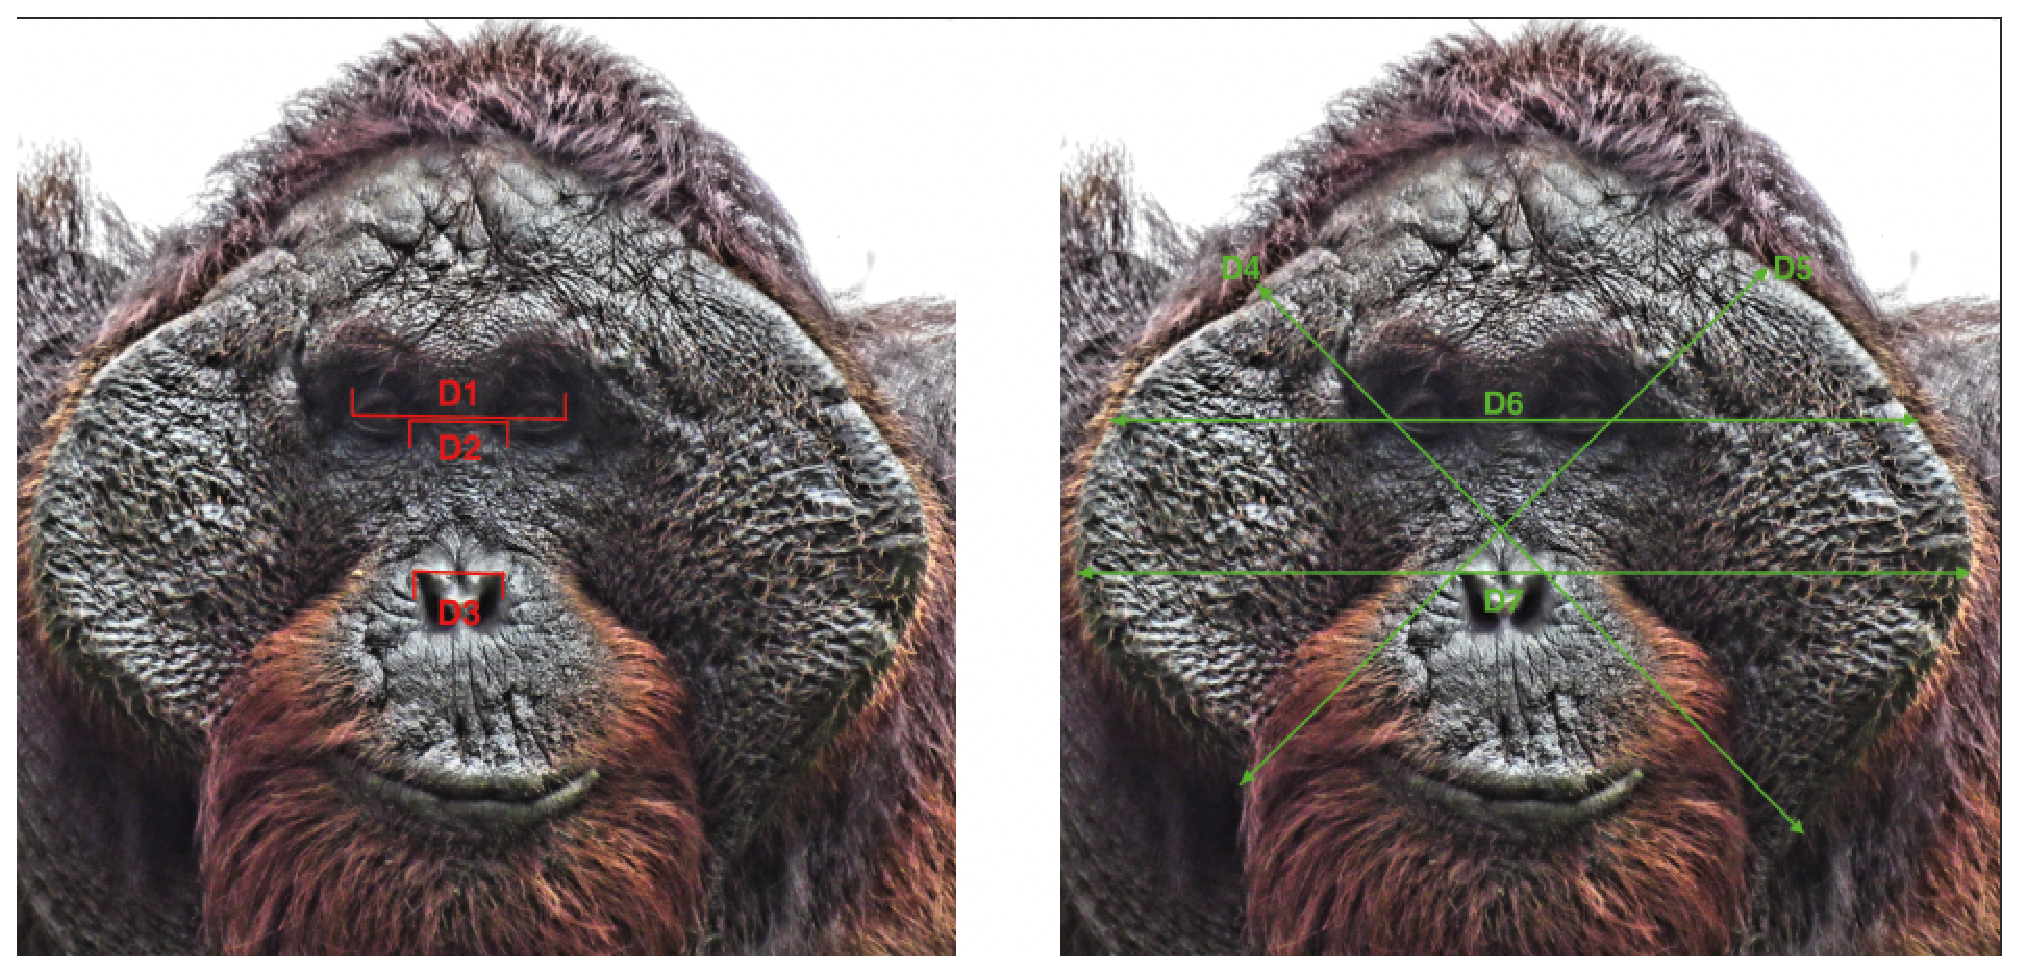
\includegraphics[width=1.0\textwidth]{Chapter2/Figs/Vector/mawasboth.eps}
    \caption{Measurements for facial symmetry and flange symmetry. }
    \label{fig:orangutanfameasures}
\end{figure}


Horizontal fluctuating asymmetry (HFA) was measured using an adaptation of the methods used in Jacobson et al. This method generates a mean x- and y-midline for each image from the mean midpoints of D1-D3. HFA was measured as the difference (pixels) of the mean midpoint of each of the horizontal lines from the midline. As the distance from each individual to the camera was unknown, the relative HFA (rHFA) scores were calculated for analysis. The relative HFA was calculated by dividing the distance (pixels) of the left LM to the midline by the distance between the left and right LM, resulting in a value of approximately 0.5 which will indicate the proportion of trait length for that side of the body. This \textit{r}HFA value will then be subtracted from 0.5 (perfect symmetry) to provide an rHFA score. A value of 0 is perfect symmetry, a negative value indicates a right-hand trait bias, and a positive value indicates a left-hand trait bias. A raw \textit{r}HFA score for a particular photo was made by summing the absolute values of these deviations. A composite \textit{r}HFA score for an individual was then made by averaging the raw \textit{r}HFA scores collected for that individual.

Vertical Fluctuating Asymmetry (VFA) was not calculated for this study, as only relative scores of FA were able to be used. This was also true for measures D4 and D5 due to their vertical components. 
To reduce the impact of confirmation bias, a random number was assigned for the first set of measurements for each photo and the measurements were obtained without knowing which site the individual was from \citep{Kozlov.2015}. Two sets of measurements were collected for each photo 1 month apart, and the same individual recorded the measurements to reduce inter-observer reliability issues.

Image analysis was performed in Fiji \citep{Schindelin.2012}.

\begin{table}[h]
\begin{center}
\begin{tabular}{l l}
\hline 
\multirow{1}{*}Measure & Definition \\
\hline
HFA scores & \(H1, H2, H3\) \\
\textit{r}HFA scores & \(\textit{r}H1 = 0.5 - \frac{\bar{H} - LM1}{H1},  \textit{ r}H2 = 0.5 - \frac{\bar{H} - LM2}{H2}, \textit{ r}H3 = 0.5 - \frac{\bar{H} - LM5}{H3}\)\\
Raw \textit{r}HFA score & \(\sum |\textit{r}H1| + |\textit{r}H2| + |\textit{r}H3|\) \\
Composite \textit{r}HFA & \(\sum \frac{\textit{r}H1_a + \textit{r}H1_b+...+\textit{r}H1_n}{n} + \frac{\textit{r}H2_a + \textit{r}H2_b+...+\textit{r}H2_n}{n}+... +\frac{\textit{r}Hn_a + \textit{r}Hn_b+...+\textit{r}Hn_n}{n}\)\\
\hline 
\end{tabular}
\caption{Explanation of the calculations used for FA analysis}
\end{center}
\end{table}

\subsection{Analysis}
To test for repeatability of FA measurements between images, a Pearson's correlation was performed on the raw \textit{r}HFA scores from two separate images of the same individual. Repeatability between replicate measurements of the same photograph was also examined using Pearson's correlations.

To test whether there is no effect of DA or AS, frequency distributions were plotted for each pair of LM to visually check for bimodal or platykurtic distributions. Additionally, a one-sample t-test and the Shapiro-Wilks test were performed on each \textit{r}FA score to test that the mean of each score was 0, and that they followed a normal distribution.

Two-way ANOVAs were performed to test whether the observed variance in \textit{r}HFA scores was due to measurement error (ME) rather than FA.  Following the recommendations of \citet{Palmer.1986} these tests were set up using the factors of Indiviudal (I), side [right or left] (S) and replicate (R) \citep{Palmer.1986} . The ratio of the I*S mean square to the combined I*S*R and I*R mean squares provides an F test of the degree of variation caused by FA as opposed to digitisation error or imaging error (I*S*R) \citep{Swaddle.1994}. An F score of >1 indicates measured FA is greater than ME.

Each individuals \textit{r}HFA measurements were correlated against each other to test whether individual scores were related to each other. The high correlation between individual \textit{r}HFA scores may indicate poor individual condition rather than the impact of external environmental factors, which are often temporary and impact individuals at different stages of development. 

Due to the inconsistent quality of photographs available in the dataset, it is important to verify the role each photograph's attributes has on ME. I plotted Pearson's correlations between ME and total resolution, focal length, and face size. The distance (pixels) between LM2 and LM3 was used as a proxy for face size. To examine the impact of the study site on composite \textit{r}HFA, a one-way mixed effect ANOVA was carried out, with Individual being used as a random effect. To test the usability of the LMs of the flange as measures of FA Shapiro-Wilks tests and t-tests were performed to examine whether signed FA values for these measurements were normally distributed with a mean of 0. Additionally, Pearson correlations and ICCs were carried out between 2 measurements from different photos. Finally, Pearson's correlations were carried out between replicate measurements of the same photo as a measure of observer reliability.

All statistical tests are two-tailed unless otherwise stated and the statistical analysis was performed in R version 4.2.2 \citep{R.2018}. 

\section{Results}

\subsection{Normality tests}

The frequency distributions of the signed FA scores were all normally distributed with a mean that did not differ significantly from 0 (Table 2), indicating that DA or AS was not observed. Pearson's correlations showed a high level of repeatability between HFA measurements.
\begin{center}
\resizebox{\textwidth}{!}{%
\begin{tabular}{l c c c l l c}
\hline
\multirow{2}{*}{Measure} & \multirow{2}{*}{Number} & \multirow{2}{*}{S-W} & \multirow{2}{*}{t-test} & \multicolumn{2}{c}{Pearson's \textit{r}} & \multirow{2}{*}{Repeatability (R)}\\ 
\cline{5-6}
& & & & Between different photos & Same photo\\
\hline
\textit{r}H1 & 24 & 0.944 & 0.053 & 0.909*** & 0.973*** &  0.907***\\

\textit{r}H2 & 24 & 0.971 & 0.181 & 0.941*** &  0.956*** & 0.942***\\

\textit{r}H3 & 24 & 0.959 & 0.721 & 0.941*** &  0.968*** & 0.938***\\

\hline 
\end{tabular}
}
\end{center}

\textit{Table 2:} Tests on facial LMs for measurement error, antisymmetry, directional symmetry, and normality using unsigned FA scores. * indicates a p-value of < 0.05, ** < 0.01, *** < 0.001.

\subsection{ANOVAs}

The two-way ANOVAs indicated that FA exceeded ME for the one HFA measurement: \(F_{H1} = (24,224) = 2.754, p < 0.001\). However, FA did not exceed the expected ME for the other two HFA measurements, \(F_{H2} = (24,226) = 1.146, p=0.289\); \(F_{H3} = (27,224) = 0.726, p=0.838\).
ANOVAs were not calculated for relative flange measurements because of their poor repeatability between replicates.

\subsection{Measurement error and factors}

A Pearson's correlation between the raw HFA scores of two different photos of the same individual indicated a high level of repeatability (\textit{r}= 0.906, N = 24, \textit{p} < 0.001).

Pearson's correlations indicated that ME was positively correlated with face size (\textit{r} = 0.661, N = 173, \textit{p} < 0.001), but was not correlated with focal length  (\textit{r} = 0.322, N = 173, \textit{p} < 0.134) or rHFA (\textit{r}= 0.291, N = 173, \textit{p} = 0.465). Face size was also not correlated with rHFA (\textit{r} = 0.389, N = 173, \textit{p} = 0.674). 

rHFA was moderately correlated with the total resolution of a photograph, however this result was not statistically significant \(r = 0.498, N = 173, p=0.0597\). There was no correlation between total resolution and imaging error \(r = 0.011, N = 173, p=0.953\)

\begin{center}
\begin{tabular}{l l l l l l l}
\hline
\multirow{1}{*}{  } & \multirow{1}{*}{\textit{r}H1} & \multirow{1}{*}{\textit{r}H2} & \multirow{1}{*}{\textit{r}H3} \\ 
\hline
\textit{r}H1 & - & 0.821*** & 0.941***  \\

\textit{r}H2 & 0.821*** & - & 0.939*** \\

\textit{r}H3 & 0.941*** & 0.939*** & - \\
\hline 
\end{tabular}
\end{center}
\textit{Table 3.} Pearson's correlation coefficients calculated for \textit{r}HFA. * indicates a p-value of < 0.05, ** < 0.01, *** < 0.001.
\subsection{Flange measurements}

Pearson's correlations between flange measurements showed moderate-high repeatability between photos. 

\begin{center}
\begin{tabular}{l c c c l l c}
\hline
\multirow{2}{*}{Measure} & \multirow{2}{*}{Number} & \multirow{2}{*}{S-W} & \multirow{2}{*}{t-test} & \multicolumn{2}{c}{Pearson's \textit{r}} & \multirow{2}{*}{Repeatability (R)}\\ 
\cline{5-6}
& & & & Between photos & Same photo\\
\hline
\textit{r}D6 & 24 & 0.927 & 0.877 & 0.648** &  0.941*** & 0.570*\\

\textit{r}D7 & 24 & 0.908 & 0.915 & 0.551* &  0.928*** & 0.462*\\
\hline 
\end{tabular}
\end{center}
\textit{Table 4:} Tests on flange LMs for measurement error, antisymmetry, directional symmetry and normality using unsigned FA scores. * indicates a p-value of < 0.05, ** < 0.01, *** < 0.001.


\begin{center}
\begin{tabular}{l l l l l}
\hline
\multirow{1}{*}{  } & \multirow{1}{*}{\textit{r}D6} & \multirow{1}{*}{\textit{r}D7}\\ 
\hline
\textit{r}D6 & - & 0.306 \\

\textit{r}D7 & 0.306 & - \\
\hline 
\end{tabular}
\end{center}
\textit{Table 5}: Pearson's correlations between flange measurements. * indicates a p-value of < 0.05, ** < 0.01, *** < 0.001.

\subsection{Differences between sites}
The average composite \textit{r}HFA score across all individuals was \(0.0342 \pm 0.0141, N = 24\). In Tuanan, the average composite \textit{r}HFA score was \(0.0381 \pm 0.0176. N = 14\), while in Sumatra the average score was \(0.0302\pm0.00931, N = 10\). A one-way mixed effect ANOVA on the impact of field site (fixed effect) and individual (random effect) on composite FA scores indicated that there was a significant difference in the mean composite FA of both field sites \(F(24,67) = 47.287, p < 0.001\). This difference was still seen when using the \textit{r}H1 as the response variable: \(F(24,67) = 6.032, p < 0.001\).

\begin{figure}[htbp!] 
\centering    
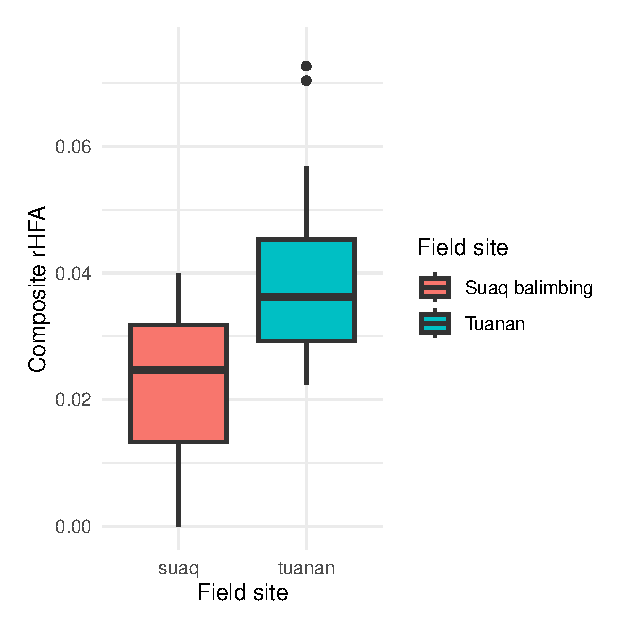
\includegraphics[width=0.6\textwidth]{Chapter2/Figs/Vector/compositefaboxplot.eps}
\caption{Variation in composite \textit{r}HFA (left) across field sites. Tuanan (Borneo) showed a significantly higher level of composite \textit{r}HFA compared to Suaq Balimbing (Sumatra), F(24,67) = 47.287, p < 0.001.}
\label{fig:Variation in composite rHFA (left) across field sites.}
\end{figure}
\section{Discussion}

The main issue with measuring fluctuating asymmetry across studies, and in particular when using photographic datasets, is accurately measuring the inherently minor variation (usually <1\% of overall trait size). This study utilised a variety of photos stretching back to 2008, so the resolution, focus, and usability varied significantly across years and individuals. These issues are exacerbated when examining arboreal primates, where there is increased distance, focal length, and variation in face orientation. However, while strict photographic selection is essential for detecting true FA, it also significantly reduces the statistical power available to detect these small deviances. This problem was exacerbated in my study due to the small sample size, 24 males across 2 sites. 

Despite only one facial HFA measure showing higher levels of FA than expected by ME, my results indicate that long-term photographic data sets can be used to examine FA. I did not observe any relationship between imaging error and total resolution, focal length, or rHFA, suggesting that there are no major issues with using older photos when examining FA over time. However, I did observe a relationship between imaging error and relative face size. This study did not scale all faces to the same size as has been done in some previous analyses by scaling the inter-pupilary distance to the same width \citep{Little.2008}. My results indicate that this is a useful step for future FA studies to minimise imaging error.

Even when scaled to the same size, the true facial size can pose a problem for FA measurements. Larger faces are more susceptible to orientation error, because minor deviations in frontal or rotational orientation are harder to assess \citep{Boulton.2013}. More studies are required to examine the impact of face size on measured FA, as currently there is no literature on the subject.

Of all of the facial LMs tested, the one that showed higher levels of FA than expected through measurement error is the outer eye tips. There are morphological reasons why this region would undergo higher levels of FA compared to other facial LMs in flanged males. The facial musculature of the orangutan forms a supporting role of the flange, in particular the M. obicularis oculi which surrounds the eye \citep{Winkler.1989}. As the flange grows, it can unevenly affect the shape of the muscle, resulting in greater FA at the outer edges of the eye tips for different individuals. As examination of non-flanged individuals was beyond the scope of this study, further examination on the differences in FA between flanged and unflanged males is needed to confirm this hypothesis. However, my results do indicate that relative facial FA can be measured on arboreal primates, subject to both a) strict photograph selection criteria, b) suitable landmark selection, and c) rigorous statistical analysis to confirm the repeatability of any measurements.

Flange measurements were significantly less repeatable and showed weaker correlation between different photographs of the same individual compared to facial measurements despite similar levels of within-photo replicability to facial LMs. There are a few potential reasons for this discrepancy. Methodologically, flange measurements may be more susceptible to measurement error compared to facial LMs. Some flanges slightly curve towards the face at the edges, and so these measurements may be more susceptible to orientation error compared to facial LMs. Additionally, as the flange has width, in instances where the face is slightly facing away from the observer, the edge of the flange will appear differently. I attempted to control for these issues with strict photo selection, however these may partially explain why these are less repeatable than facial LMs. However, there may be morphological reasons for this observed difference. The flanges are mainly made up of fat bound to fibro-fatty tissues \citep{Winkler.1989}. Under severe negative energy balance, this tissue can be used for energy under ketosis. As a result, this may cause fluctuation in flange size over the year, and if this effect is caused by nutritional deficiency, I would expect this to show a time-lagged correlation with fruit availability. I will explore this hypothesis in Chapter 3. 


\subsection{Why is FA in Tuanan greater than Suaq Balimbing?}
The results indicate that male orangutans in Tuanan experience higher levels of fluctuating asymmetry compared to Suaq Balimbing. Given the relatively minor size of the effect and that there was only one FA measure where the FA exceeded ME, it is important not to overstate the significance of the results. However, there are significant ecological differences between the two sites that may contribute to the observed differences. 
Firstly, Suaq Balimbing has the highest level of consistent fruit availability compared to any other orangutan field site \citep{Singleton.2001}. Many orangutans live in forests characterised by a large variation in fruit availability, which can lead them to fall into periods of severe negative energy balance, and the unusually high productivity of Suaq shields native orangutans from the worst of these effects. This is in part due to a wider difference in soil quality between Sumatra and Borneo due to the presence of 34 active volcanoes on Sumatra, which Borneo lacks \citep{Barber.2005}.
Second, is the ecological health of each study site. Suaq Balimbing is in the Gunung leuser National Park, which has been a protected area since colonial times and formally made a national park in 1980 \citep{Singleton.2001}. There has been minimal human intrusion into the habitat and illegal logging is uncommon. However, Tuanan Research station lies within the area that was part of the now defunct Mega Rice Project that was active from 1996-1997 \citep{Erb.2018}. As a result, this area was selectively logged in the 1990s for commercial purposes before becoming a protected area in 2003, and the area is still recovering \citep{Husson.2008}. Tropical forest fragments can recover relatively quickly from low-intensity land use; however, recovery rates vary across metrics. Recovery to 90\% of old growth values for structure and species diversity can take up to 60 years, while recovery of species composition and biomass can take over 120 years \citep{Poorter.2021}. As such, the altered community composition of the forest may exacerbate existing periods of negative energy balance due to the diminished diversity of food sources. 
Adding to this is the asymmetric impact of fires in these two communities. Borneo has experienced multiple large-scale fires, most famously the 1997 fires across 0.73Mha of forested peatland, which released between 0.81 and 2.57Gt of carbon into the atmosphere \citep{Page.2002}. These fires are made more common due to the impacts of global change and climate change, in particular the increase in the strength of El niño events; and land use change over the areas burnt \citep{Collins.2019, Siegert.2001}. These fires are part of a dangerous positive feedback loop, as previous studies have indicated that recently logged forest fragments suffer more severe damage during fire outbreaks \citep{Siegert.2001}. Additionally, areas that have recently burnt are more likely to burn again soon due to the large amount of dead flammable wood left over from large burns \citep{Cochrane.1999}. Tuanan has undergone multiple burns, including the 1997 event and most recently from March 2015 to January 2016; whereas in contrast, no fires have been recorded at Suaq Balimbing. Studies since the 2015 outbreak have indicated that fire has significant direct and indirect negative impacts on orangutans. Exposure to hazardous concentrations of \(PM_{10}\) particulate matter decreases the daily distance travelled and increases fat catabolism \citep{Erb.2018}. The secondary effects of fires are severe reduction in fruit availability, following a prolonged smoke cover period causing significantly lower overall fruit availability compared to regular annual decreases, which also causes decreased movement and increased fat catabolism \citep{Ashbury.2022}.
Given the data set of exclusively flanged males, it is difficult to distinguish the causes of the observed differences in FA between the two sites; however, future studies in the area could establish the impact of the fire on juveniles and infants by examining facial FA before and after the fire.

In summary, my results highlight the use of historic data sets for measuring facial FA and establishing differences across populations, subject to strict selection criteria, suitable landmark choice, and large sample sizes.

\nomenclature[z-DI]{DI}{Developmental Instability}
\nomenclature[z-FA]{FA}{Fluctuating Asymmetry}
\nomenclature[z-HFA]{HFA}{Horizontal Fluctuating Asymmetry}
\nomenclature[z-VFA]{VFA}{Vertical Fluctuating Asymmetry}
\nomenclature[z-DA]{DA}{Directional Asymmetry}
\nomenclature[z-AS]{AS}{Antisymmetry}
\nomenclature[z-ME]{ME}{Measurement Error}

